\section{Explanation of terms}\label{explanationofterms}

In this section we explain some of the phrases, words and terms used through out the article so the 
readers unfamiliar with version control might get an overall idea what version control is about.

We will often refer to CVS\footnote{http://www.nongnu.org/cvs/} (Concurrent Versions System) and SVN\footnote{http://subversion.apache.org/} (Subversion) which are the most used centralized Version Control Systems.

It is also noteworthy that the term “Revision Control System (RCS)” may be used instead of “Version Control System (VCS)”. These two are interchangeable. In other books and articles revision control may also be referred to as “Software Configuration Management (SCM)” or “Source code control”. Those terms have different meanings in different contexts and there is an ongoing discussion about the definitions of those terms. \cite[chapter 1]{hgbook2009}

\subsection{Repository}

A repository in DVCS terms is a folder which can contain sub folders and files of all categories. 
This folder is tracked by the DVCS so there is a history for every file containing whether it was renamed, deleted or changed. 
How these changes are tracked is different from system to system. CVS for example “isolates” 
files and handles them individually. So each file has its own version number. If a file gets changed, CVS will 
save the delta (i.e. what has changed) and give the file a new number. SVN does it a little bit 
different. If a file gets changed and commited, the whole repository gets a new version number, usually counting from 1, 2 to n. 
In SVN terms such a version of the repository is referred to as a “revision”.

Git also handles the repository as a whole. It saves each new file version as a whole and not just the delta as SVN and CVS does. 
In Git there are no incrementing version numbers, instead Git uses the SHA-1 checksum. For each file there is such a 
checksum and the checksum which represents a certain revision is a sum of these checksums. \cite[chapter 2.3]{gitpro2009}
This explanation is a good approximation for those unfamiliar with version control.


\subsection{Commit}

Committing means that changes being made to some files inside the repository get permanent. 
After committing the repository has a new revision number. It is possible to move back and forth between commits enabling developers to work 
from an older version if a bug tied up the functionality of the application.

Usually with each commit there is some meta information saved like, who has committed and what has been done since the last commit. 
It is good practice to give detailed information about what files have changed and the purpose of these changes, so others working 
on the repository know whats going on.


\subsection{Checkout}

In CVS and SVN a checkout is the operation of creating a local working copy of a certain version from the 
central repository. In Git checkout has a slightly different meaning. Creating a local working copy in Git is 
called “clone”. \cite[chapter 2.1]{gitpro2009} Checkout is called the operation of switching between different versions and branches. I.e. 
the local working copy is changed to another version. \cite[chapter 3.2]{gitpro2009}


\subsection{Branch}

Branching means that development diverges from the main line and continues without messing it up. Branches are a feature where Git really shines 
because they are very lightweight and really fast compared to other VCSs. \cite[chapter 3]{gitpro2009}

\begin{figure}[ht]
  \centering
  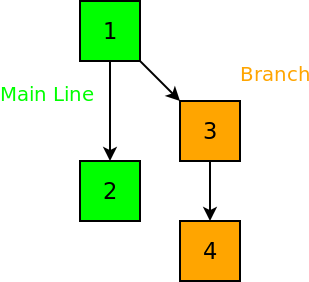
\includegraphics[width=0.4\textwidth]{img/Gen_Branch}
  \caption{Basic branching}
  \label{fig:gen_branch} 
\end{figure}

Figure \ref{fig:gen_branch} shows an example of how such a branch could look like. Version 1 in 
this example is the initial commit with some files. Now developer A continues development in the main line by fixing 
some bugs and improving the current version. Developer B now wants to add some new experimental 
features to version 1. Because developer B does not want to mess up the hopefully stable main line and the 
changes of developer A, he creates a branch where he can develop the new features until they are stable. 
So the versions 3 and 4 are the branch and the versions 1 and 2 are the stable main line.


\subsection{Merge}

Merging is the process of integrating changes to a file which was modified by two people individually 
at the same time. When there are no conflicts the merge can be done automatically, else, a person must resolve 
the conflict. A conflict can occur when both people change the same lines inside a file, so the person who 
merges the changes must decide which version to use or how to integrate both versions into the file.

“Merging branches” means that the changes made to a branch will be merged into another branch. 
To successfully merging branches they must have a common parent in their history.

\begin{figure}[ht]
  \centering
  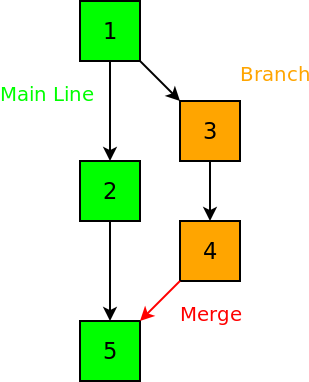
\includegraphics[width=0.4\textwidth]{img/Gen_Merge}
  \caption{Basic merging}
  \label{fig:gen_merge} 
\end{figure}

Figure \ref{fig:gen_merge} shows a later stage of the example from above. The developers decide that 
the new features in version 4 are stable and can be merged into the main line.


\subsection{Tagging}

Tagging means marking a certain version or revision with a tag. 
Assigning a tag to a version is just for convenience, normally it is used to tag important project milestones. 
For example if the application reaches version 1.5, one can assign a tag named “v1.5” 
to the commit or revision which was used to build the “application 1.5” or which represents the “application 1.5”. 
This way it will be very easy to find the commit needed in the future if an older version of the application should be built.

\begin{figure}[ht]
  \centering
  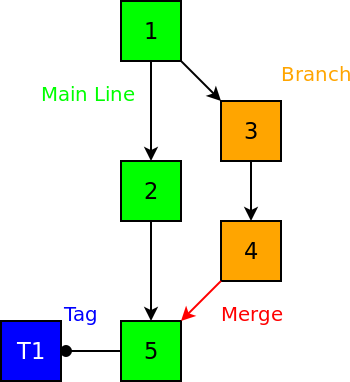
\includegraphics[width=0.4\textwidth]{img/Gen_Tag}
  \caption{Basic tagging}
  \label{fig:gen_tag}
\end{figure}

Figure \ref{fig:gen_tag} shows how the new version 5 from above is tagged with a tag T1.
